% This work is licensed under the Creative Commons
% Attribution-NonCommercial-ShareAlike 4.0 International License. To view a copy
% of this license, visit http://creativecommons.org/licenses/by-nc-sa/4.0/ or
% send a letter to Creative Commons, PO Box 1866, Mountain View, CA 94042, USA.

\section{Argmin-Theoreme in \texorpdfstring{$C(\R)$}{C(R)}} %8
Erinnere an folgende Probleme, vergleiche Gleichungen \eqref{eq1.2} und \eqref{eq1.5} in Kapitel 1 zum Median.\\
Wann überträgt sich die Konvergenz (f.s. oder in Verteilung) von stetigen stochastischen Prozessen auf deren Minimalstellen?

\begin{definition}\label{definition8.1}
	Sei $f\in C(\R)$.
	\begin{enumerate}[label=(\arabic*)]
		\item $\begin{aligned}
			A(f):=\argmin(f):=\left\lbrace t\in\R:f(t)=\inf\limits_{s\in\R} f(s)\right\rbrace
		\end{aligned}$ = Menge aller Minimalstellen
		\item $\tau\in A(f)$ heißt \textbf{wohl-separiert} 
		\begin{align*}
			:\Longleftrightarrow\inf\Big\lbrace f(t):|t-\tau|\geq\varepsilon\Big\rbrace>f(\tau)\qquad\forall 0<\varepsilon\in\Q
		\end{align*}
	\end{enumerate}
\end{definition}

\begin{bemerkungnr}\label{bemerkung8.2}\
	\begin{enumerate}[label=(\arabic*)]
		\item $A(f)\neq\emptyset$ ist natürlich nicht ausgeschlossen, aber in jedem Fall ist $A(f)$\\ \underline{abgeschlossen} in $\R$, denn:\\
		Sei $(t_n)_{n\in\N}\subseteq A(f)$ mit $t_n\stackrel{n\to\infty}{\longrightarrow}t.$ Dann gilt:
		\begin{align*}
			f(t)&=\limn\underbrace{f(t_n)}_{=\inf\limits_{s\in\R}f(s)}=\inf\limits_{s\in\R}f(s)
			\implies t\in A(f)
		\end{align*}
		\item $\tau$ wohl-separariert $\implies\tau$ eindeutig, denn:\\
		Sei $\tilde{\tau}\in A(f)$ und $\tilde{\tau}\neq\tau$. Also:
		\begin{align}\label{eqBemerkung8.2Stern}\tag{$\ast$}
			\exists 0&<\varepsilon\in\Q:\big|\tau-\tau|>\varepsilon\\\nonumber
			\inf\limits_{s\in\R}f(s)
			\overset{\tilde{\tau}\in A(f)}&=
			f(\tau)
			\overset{\eqref{eqBemerkung8.2Stern}}{\geq}
			\inf\Big\lbrace f(t):|t-\tau|\geq\varepsilon\Big\rbrace
			\overset{\tau\text{ wohl-sep}}{\geq}
			f(\tau)
			\overset{\tau\in A(f)}{=}
			\inf\limits_{s\in\R} f(s)
		\end{align}
		Dies ist ein Widerspruch!
		\item Wohl-Separiertheit ist also eine stärkere Bedingung als Eindeutigkeit der Minimalstelle.
		Sie schließt "degenerierte" Fälle wie in Abbildung \ref{AbbMinimalstelleEindeutigNichtWohlsepariert} aus.
	\end{enumerate}
\end{bemerkungnr}

\begin{beisp}
	Wann ist eine Minimalstelle eindeutig, aber nicht wohlsepariert?
	\begin{figure}[H]
		\begin{center}
			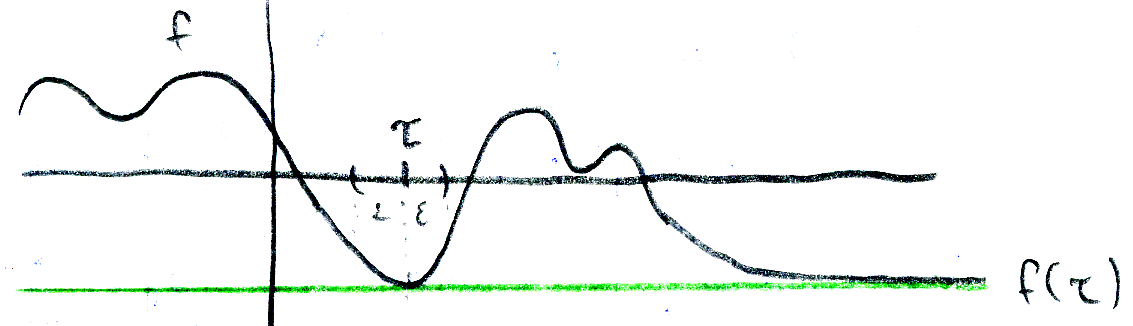
\includegraphics[width=1\textwidth]{./pics/MSTAT003.png}
            \caption{$\tau$ eindeutig, aber das Infimum von $f$ außerhalb von $(\tau-\varepsilon,\tau+\varepsilon)$ ist auch $f(\tau)$!}
			\label{AbbMinimalstelleEindeutigNichtWohlsepariert}
		\end{center}
	\end{figure}
\end{beisp}

\begin{satz}\label{satz8.3}
	Seien $f,f_n,n\in\N$ aus $C(\R)$, $\tau_n\in A(f_n)\neq\emptyset~\forall n\geq N_0\in\N$ 
	(also $\tau_n$ ist eine Minimalstelle, ab einem gewissen Zeitpunkt $N_0$.)
	und $\tau\in A(f)$ sei wohl-separiert.
	Falls
	\begin{align}\label{eqSatz8.3_1}\tag{1}
		\big\Vert f_n-f\big\Vert\overset{\text{Def}}{=}\sup\limits_{t\in\R}\big|f_n(t)-f(t)\big|\overset{n\to\infty}{\longrightarrow}0
	\end{align}
	so folgt
	\begin{align*}
		\tau_n\overset{n\to\infty}{\longrightarrow}\tau
	\end{align*}
\end{satz}

\begin{proof}
	Sei $0<\varepsilon\overset{\text{oBdA}}{\in}\Q$. Es folgt:
	\begin{align*}
		s(\varepsilon)&:=\inf\limits\big\lbrace f(t):|t-\tau|\geq\varepsilon\big\rbrace
		\overset{\text{Def wohl-sep}}{>}
		f(\tau)\\
		\implies
		\delta&:=\delta(\varepsilon):=\frac{1}{3}\cdot\big(s(\varepsilon)-f(\tau)\big)>0\\
		\overset{\eqref{eqSatz8.3_1}}{\implies}
		\exists n_0&=n_0(\delta)\in\N:\forall n\geq n_0:
		\Vert f_n-f\Vert\leq\delta
	\end{align*}
	Für alle $n\geq\max\limits(N_0,n_0)$ gilt:\\
	Falls $t\in\R$ mit $|t-\tau|\geq\varepsilon$, so folgt:
	\begin{align*}
		f_n(t)-f_n(\tau)
		&=\underbrace{f_n(t)-f(t)}_{\geq\underbrace{-\underbrace{\Vert f_n-f\Vert}_{\leq\delta}}_{\geq-\delta}}+\underbrace{\underbrace{f(t)}_{\geq s(\varepsilon)}-f(\tau)}_{\geq s(\varepsilon)-f(\tau)=3\delta}+\underbrace{f(\tau)-f_n(\tau)}_{\geq-\delta}\\
		&\geq-\delta+3\cdot\delta-\delta\\
		&=\delta>0
	\end{align*}
	Es folgt
	\begin{align}\label{eqProofSatz8.3Stern}\tag{$\ast$}
		f_n(t)>f_n(\tau)\qquad\forall t\in\R\mit|t-\tau|\geq\varepsilon
	\end{align}
	Folglich gilt $|\tau_n-\tau|<\varepsilon$, denn sonst folgte aus \eqref{eqProofSatz8.3Stern}, dass
	$f_n(\tau_n)>f_n(\tau)$ im Widerspruch zu $\tau_n$ ist Minimalstelle von $f_n$.\\
	Somit gezeigt:
	\begin{align*}
		\forall\varepsilon\in\Q\cap(0,\infty):\exists m_0=m_0(\varepsilon):=\max\limits(N_0,n_0):\forall n\geq m_0:|t_n-\tau|<\varepsilon
	\end{align*}
\end{proof}

Satz \ref{satz8.3} lässt sich problemlos von $\R$ auf offene Intervalle $I=(a,b)$ übertragen.\nl
Für kompakte Intervalle $I=[a,b]$, $a<b\in\R$ muss $\tau$ nur eindeutig sein.
Es gilt:

\begin{satz}\label{satz8.4}
	Sei also $I=[a,b]$ kompaktes Intervall und seien $f,f_n,n\in\N$ aus $C(I)$. 
	Dann gilt:
	\begin{enumerate}[label=(\arabic*)]
		\item $\begin{aligned}
			A(f_n)\neq\emptyset\qquad\forall n\in\N
		\end{aligned}$
		\item Falls $\tau$ \underline{eindeutige} Minimalstelle von $f$ ist und falls
		\begin{align*}
			\Vert f_n-f\Vert_I:=\sup\limits_{t\in I}\big|f_n(t)-f(t)\big|\overset{n\to\infty}{\longrightarrow}0
		\end{align*}
		so gilt für \underline{jede} Auswahl $\tau_n\in A(f_n)$:
		$\tau_n\overset{n\to\infty}{\longrightarrow}\tau$
	\end{enumerate}
\end{satz}

%Ferger: "In irgendeinem der Seminarräumen ist mal eine Tafel von der Wand gefallen. Und ich möchte jetzt nicht unter so einer Tafel begraben liegen.
% Vielleicht ist das für einen Professor ein schöner Tod. Aber bitte jetzt noch nicht."
% "Ich bin ja von Natur aus etwas ängstlich. Es gab da mal so ein lustiges Lied und da singt der Sänger: "Leute seid nicht feige, lasst mich ...""

\begin{proof}
	\underline{Zeige (1):}\\
	Folgt, da jede stetige Funktion auf einem Kompaktum das Infimum annimmt.\nl
	\underline{Zeige (2):}\\
	$\tau$ ist wohl-separiert auf $I$, denn: 
	Angenommen, es wäre nicht so, also angenommen
	\begin{align*}
		\exists0<\varepsilon\in\Q:\inf\limits\big\lbrace f(t):t\in I:|t-\tau|\geq\varepsilon\big\rbrace=f(\tau)
	\end{align*}
	Die Menge $K_\varepsilon:=\lbrace t\in I:|t-\tau|\geq\varepsilon\rbrace$ ist kompakt.  
	Weil $f$ stetig ist, nimmt $f$ auf $K_\varepsilon$ ihr Infimum an, d.h.
	\begin{align*}
		\exists\sigma\in I:|\sigma-\tau|\geq\varepsilon\mit f(\sigma)=\inf\limits
		\big\lbrace f(t):t\in I:|t-\tau|\geq\varepsilon\big\rbrace
		=f(\tau)
	\end{align*}
	Also ist $\sigma$ eine \underline{weitere} Minimalstelle von $f$ (denn $\sigma$ und $\tau$ haben positiven Abstand zueinander) im Widerspruch zur Eindeutigkeit von $\tau$.\\
	Jetzt weiter wie im Beweis von Satz \ref{satz8.3}.
\end{proof}

Es ergeben sich nun mühelos Argmin-Theoreme für fast sichere Konvergenz:

\begin{satz}\label{satz8.5}
	Seien $M=\big\lbrace M(t):t\in \R\big\rbrace,M_n=\big\lbrace M_n(t):t\in \R\big\rbrace,n\in\N$ stochastische Prozesse über $(\Omega,\A,\P)$ mit Pfaden in $C(\R)$ (d.h. $M\colon \R\to\R,~t\mapsto M(t,\omega)$ stetig für alle $\omega\in\Omega$).
	Es gelte:
	\begin{enumerate}[label=(\arabic*)]
		\item $\begin{aligned}
			\tau(\omega)\in A\big(M(\cdot,\omega)\big)\overset{\Def}{=}
			\argmin\big(M(\cdot,\omega)\big)
			\overset{\Def}{=}\set{t\in R:\inf\limits_{s\in\R}M(s,\omega)=M(t,\omega)}
		\end{aligned}$ f.s.\\
		für eine Zufallsvariable $\tau\colon\Omega\to\R$, also $\P\big(\big\lbrace\omega\in\Omega:\tau(\omega)\in A\big(M(\cdot,\omega)\big)\big\rbrace\big)=1$
		\item $\begin{aligned}
			\inf\limits\big\lbrace M(t):|t-\tau|\geq\varepsilon\big\rbrace>M(\tau)\text{ f.s.}\qquad\forall 0<\varepsilon\in\Q
		\end{aligned}$ (wohl-separiertheit)
		\item $\begin{aligned}
			\norm[\big]{M_n-M}_\infty\overset{n\to\infty}{\longrightarrow}0\text{ f.s.}
		\end{aligned}$
	\end{enumerate}
	Dann gilt für jede Folge $(\tau_n)_{n\in\N}$ von Zufallsvariablen mit $\tau_n\in A(M_n)$ f.s.:
	$\tau_n\overset{n\to\infty}{\longrightarrow}\tau$ f.s.
\end{satz}

\begin{proof}
	Setze
	\begin{align*}
		\Omega_0:=\underbrace{\Big\lbrace\omega\in\Omega:\tau(\omega)\in A\big(M(\cdot,\omega)\big)\Big\rbrace}_{=:\big\lbrace\tau\in A(M)\big\rbrace\text{ Einsmenge wg (1)}}
		&\cap\bigcap\limits_{0<\varepsilon\in\Q}
		\overbrace{\underbrace{\Big\lbrace\inf\limits\big\lbrace M(t):|t-\tau|\geq\varepsilon\big\rbrace>M(\tau)\Big\rbrace}_{\text{Einsmenge wg. (2)}}}^{\hat{=}\text{wohl-separiert}}\\
		&\cap\underbrace{\Big\lbrace\Vert M_n-M\Vert\overset{n\to\infty}{\longrightarrow}0\Big\rbrace}_{\text{Einsmenge wg (3)}}
		\cap\bigcap\limits_{n\geq1}\underbrace{\Big\lbrace\tau_n\in A(M_n)\Big\rbrace}_{\text{Einsmenge nach Vor.}}
	\end{align*}
	Erinnerung: Abzählbare Schnitte von Einsmengen sind Einsmengen.\\
	Dann gilt $\P(\Omega_0)=1$. 
	Da $\Omega_0\overset{\ref{satz8.3}}{\subseteq}\big\lbrace\tau_n\overset{n\to\infty}{\longrightarrow}\tau\big\rbrace$, folgt die Behauptung.
\end{proof}

Analog erhält man mit Satz \ref{satz8.4}:

\begin{satz}\label{satz8.6}
	Seien $M,M_n,n\in\N$ stochastische Prozesse über $(\Omega,\A,\P)$ mit Pfaden in $C(I)$,
	wobei $I$ kompaktes Intervall ist.
	Es gelte:
	\begin{enumerate}[label=(\arabic*)]
		\item Es gibt eine Zufallsvariable $\tau$, die f.s. eindeutige Minimalstelle von $M$ ist.
		\item $\begin{aligned}
			\Vert M_n-M\Vert_I\overset{n\to\infty}{\longrightarrow}0
		\end{aligned}$ f.s.
	\end{enumerate}
	Dann gilt für jede Folge $(\tau_n)_{n\in\N}$ von Zufallsvariablen mit $\tau_n\in A(M_n)$ f.s.:
	$\tau_n\overset{n\to\infty}{\longrightarrow}\tau$ f.s.
\end{satz}

\begin{proof}
	Setze
	\begin{align*}
		 \Omega_0&:=\lbrace\tau\text{ ist eindeutige Minimalst. v. }M\rbrace
		 \cap\Big\lbrace\Vert M_n-M\Vert_I\overset{n\to\infty}{\longrightarrow}0\Big\rbrace
		 \cap\bigcap\limits_{n\geq1}\Big\lbrace\tau_n\in A(M_n)\Big\rbrace\\
		 &\implies\P(\Omega_0)=1
	\end{align*}		
	Da $\Omega_0\overset{\ref{satz8.4}}{\subseteq}\Big\lbrace\tau_n\overset{n\to\infty}{\longrightarrow}\tau\Big\rbrace$, folgt die Behauptung.
\end{proof}

\subsection{Anwendung in der Statistik} %nonumber
Maximum-Likelihood-Schätzung in 1-parametrigen Exponentialfamilien
Seien $(X_n)_{n\geq1}$ i.i.d. Kopien von Zufallsvariablen $X$, (d.h. $X_i\sim X$ bzw. $X_i\overset{\L}{=}X$)
mit Werten im Messraum $(\X,\F)$ und mit $\mu$-Dichte 
\begin{align*}
	f_\theta(x)&=c(\theta)\cdot h(x)\cdot\exp\big(q(\theta)\cdot T(\theta)\big)
	\qquad\forall x\in\X,\theta\in\Theta\subseteq\R
\end{align*}

% Ferger:
% In der Statistik werden Beobachtungen als Realisierungen von Zufallsvariablen aufgefasst, also X(\omega)=Beobachtung für ein \omega\in\Omega
% X_i kann das Befragungsergebnis des $i$-ten Probanden sein
% Kann man die $X_i$ in der Theorie als Unabhhängigkeit annehmen? -> siehe Zeitreihenanalyse
% Natürlich ist es nicht immer gegeben, unabhängige Daten zu betrachten. Mann muss sich in jeder Situation fragen, ob diese Modellierung sinnvoll ist.

% Ferger zu mir: "Schreiben Sie auch meine Späße mit?"
% Ich: "Ja, natürlich!"
% Ferger: "Das ist bedenklich..."

Erinnere an Maximum-Likelihood-Schätzer (MLS /MLE):
\begin{align*}
	\ul{X}_n:=\big(X_1,\ldots,X_n\big)
\end{align*}
hat \textbf{Likelihood-Funktion}
\begin{align*}
	L_n(\theta,\ul{X}_n)&:=\prod\limits_{i=1}^n L\big(\theta,X_i\big)
	\qquad\mit\qquad
	L(\theta,x):=f_\theta(x)
\end{align*}
Zugehörige \textbf{$\log$-Likelihood-Funktion} ist
\begin{align*}
	l_n\big(\theta,\ul{X}_n\big)&:=\log\Big(L_n\big(\theta,\ul{X}_n\big)\Big)
	=\sum\limits_{i=1}^n\log\big(\theta,X_i\big)
	=\sum\limits_{i=1}^n l\big(\theta,X_i\big)\qquad\mit
\\
l(\theta,x)&:=\log\big(L(\theta,x)\big)=\log\big(f_\theta(x)\big)
\end{align*}
Der MLS für $\theta$ ist definiert durch
\begin{align*}
	\hat{\theta}_n
	:=\argmax\limits_{\theta\in\Theta}L_n\big(\theta,\ul{X}_n\big)
	%\overset{x\mapsto\log(x)\text{ streng monoton wachsend}}{=}
	\overset{(\ast)}{=}
	\argmax\limits_{\theta\in\Theta} l_n\big(\theta,\ul{X}_n\big)
	=\argmin\limits_{\theta\in\Theta}\underbrace{-\frac{1}{n}\cdot  l_n\big(\theta,\ul{X}_n\big)}_{=:S_n(\theta)}
\end{align*}
Die $(\ast)$-Gleichheit gilt, weil $x\mapsto\log(x)$ streng monoton wachsend und stetig ist.
\begin{align*}
	l(\theta,x)&=\log\big(c(\theta)\big)+\log\big(h(x)\big)+q(\theta)\cdot T(x)\\
	\implies S_n(\theta)&=-\log\big(c(\theta)\big)\underbrace{-\frac{1}{n}\cdot\sum\limits_{i=1}^n\log\big(h(X_i)\big)}_{\text{hängt \ul{nicht} von $\theta$ ab}}-q(\theta)\cdot\underbrace{\frac{1}{n}\cdot\sum\limits_{i=1}^n T(X_i)}_{=:\overline{T}_n}\\
	&=\underbrace{-\Big(\log\big(c(\theta)\big)+q(\theta)\cdot\overline{T}_n\Big)}_{=:M_n(\theta)}-\frac{1}{n}\cdot\sum\limits_{i=1}^n\log\big(h(X_i)\big)\\
	\implies\hat{\theta}_n
	&=\argmin\limits_{\theta\in\Theta} M_n(\theta)
\end{align*}

% Ferger zu den Schülern von Uni-Live: "Ich mach' auch sonst keine Späße. Und die Studenten sind auch immer leise."
%Ferger: "Ich komme aus einem 400-Einwohner Dorf."

\textbf{Annahme:}
\begin{enumerate}[label=(\arabic*)]
	\item $\Theta\subseteq\R$ ist kompaktes Intervall
	\item $q$ ist stetig auf $\Theta$ ($\implies c$ stetig, $c>0$).
	\item Sei $\theta_0$ der \textbf{wahre} Parameter, d.h. $X_i\sim f_{\theta_0}$
\end{enumerate}

Ziel: Zeige
\begin{align*}
	\hat{\theta}_n\overset{n\to\infty}{\longrightarrow}\theta_0
	\quad\P\text{-fast sicher}
	\qquad\forall \theta_0\in\Theta
\end{align*}
Das ist die sogenannte \textbf{starke Konsistenz} der Schätzerfolge $(\hat{\theta}_n)_{n\in\N}$.

% Ferger zu den Schülern: "Liebe Kinder, bitte nicht rauchen! Rauchen ist ungesund."
%Ferger: "Ich rauche in meinem Zimmer. Das ist verboten. Da ist ziviler ungehorsam. Ich warte immer noch, dass jemand zu mir kommt und sagt, dass das verboten. Und jetzt? Werfen Sie mich jetzt raus?
% Ich habe auch einen Hund in meinem Zimmer. Ist auch verboten."

Gemäß SGGZ gilt:
\begin{align}\label{eqUnderStarkeKonsistenz}
	\overline{T}_n\overset{n\to\infty}{\longrightarrow}&\E_{\theta_0}\big[T(X)\big]\quad\P\text{-fast sicher}\\
	\E_{\theta_0}\big[T(X)\big]
	&=\int\limits_\Omega T(X)\d\P_{\theta_0}
	\overset{\eqref{eqTrafo}}{=}
	\int\limits_{\X}T(x)\underbrace{\P_{\theta_0}\circ X^{-1}}_{\text{hat $\mu$-Dichte}}(\d x)	
	\int\limits_{\X}T(x)\cdot f_{\theta_0}(x)~\mu(\d x)\nonumber
\end{align}

Erinnerung: 
\begin{align*}
	X_i:\big(\Omega,\A,\P_\theta)\to\big(\X,\F)
	\qquad
	X_i(\omega)\in\X\overset{\text{z.B.}}{=}\R
	\qquad
	\underline{X}_n:=\big(X_1,\ldots,X_n\big):\Omega\to\X^n
\end{align*}

Aus \eqref{eqUnderStarkeKonsistenz} folgt:
\begin{align*}
	M_n(\theta)\overset{n\to\infty}&{\longrightarrow}
	\underbrace{-\Big(\log\big(c(\theta)\big)+q(\theta)\cdot\E_{\theta_0}\big[T(X)\big]\Big)}_{=:M(\theta)=:M_{\theta_0}(\theta)}
	\quad\P\text{-f.s.}
	\qquad\forall\theta_0\in\Theta\\
	\Big|M_n(\theta)-M_{\theta_0}(\theta)\Big|
	&=\bigg|q(\theta)\cdot\Big(\overline{T}_n-\E_{\theta_0}\big[T(X)\big]\Big)\bigg|\\
	\implies
	\sup\limits_{\theta\in\Theta}\Big|M_n(\theta)-M_{\theta_0}(\theta)\Big|
	&=\underbrace{\left(\sup\limits_{\theta\in\Theta}\big|q(\theta)\big|\right)}_{=:c<\infty}
	\cdot\underbrace{\bigg|\Big(\overline{T}_n-\E_{\theta_0}\big[T(X)\big]\Big)\bigg|}_{\overset{n\to\infty}{\longrightarrow}0\text{ f.s.}}
\end{align*}
Die Bedingung (2) in Satz \ref{satz8.6} ist also erfüllt.

% Ferger hat am 18.01. Geburtstag

Falls $\theta_0$ eindeutige Minimalstelle von $M_{\theta_0}$ ist, so liefert Satz \ref{satz8.6} die starke Konsistenz von $(\hat{\theta}_n)_{n\in\N}$.
Zusammenfassung in:

\begin{satz}\label{satz8.7}
	 Im Modell (Exponential-Familie) sei $\Theta\subseteq\R$ kompaktes Intervall,
	 $q$ sei stetig und der wahre Parameter $\theta_0$ sei eindeutige Minimalstelle der Funktion
	 \begin{align*}
	 	M_{\theta_0}(\theta)
	 	&=-\log\big(c(\theta)\big)-q(\theta)\cdot c(\theta)\cdot\int\limits T(x)\cdot h(x)\cdot\exp\big(q(\theta_0)\cdot T(x)\big)~\mu(\d x)
	 	\qquad\forall\theta\in\Theta
	 \end{align*}
	 (Das ist eine implizite Forderung an die Verteilungsannahmen (VA).)
	 Und sei 
	 \begin{align*}
	 	\hat{\theta}_n=\argmin\limits_{\theta\in\Theta} M_n(\theta)
	 	\qquad\mit\qquad
	 	M_n(\theta)=-\log\big(c(\theta)\big)-q(\theta)\cdot\frac{1}{n}\cdot\sum\limits_{i=1}^n T(X_i)
	 \end{align*}
	 Dann gilt:
	 \begin{align*}
	 	\hat{\theta}_n\overset{n\to\infty}{\longrightarrow}
	 	\theta_0\quad\P\text{-f.s.}\qquad\forall\theta_0\in\Theta
	 \end{align*}
\end{satz}

\begin{proof}
	Folgt aus Satz \ref{satz8.6}.
\end{proof}

%Ferger: "Stellen wir uns mal konkret einen Hilbertraum vor."

Vom theoretischen Standpunkt aus ist die Kompaktheitsannahme an $\Theta$ sehr stark.
Allerdings ist dies für den Anwender keine signifikante Einschränkung.
Dafür aber neben der Stetigkeit von $q$ \underline{keine} weitere "Glattheitsannahmen".
Sind solche Glattheitsannahmen aber gegeben, so lässt sich zeigen, dass $\theta_0$ tatsächlich eindeutiger (und im Fall $\Theta=\R$ wohl-separierte) Minimalstelle von $M_{\theta_0}$ ist. 

\subsection{Anwendung in der Change-Point-Analyse} %8.2
Betrachten des Change-Point-Modell aus Kapitel 7.1:
$X_{1,n},\ldots,X_{n,n},n\in\N$ seien unabhängige reelle Zufallsvariablen mit 
\begin{align*}
	\left\lbrace\begin{array}{ll}
		X_{i,n}\text{ i.i.d }\sim(\mu,\sigma^2), &\falls 1\leq i\leq\tau_n\\
		X_{i,n}\text{ i.i.d }\sim(\nu,\tau^2), &\falls \tau_n< i\leq\tau_n\\
	\end{array}\right.,\qquad\mu\neq\nu
\end{align*}
Mit $\tau_n\in\big\lbrace1,\ldots,n-1\big\rbrace$ unbekannter \textbf{Wechselzeitpunkt}.
\begin{align*}
	\underbrace{X_1,\ldots,X_{\tau_n}}_{\text{pre-change variables}},\underbrace{X_{\tau_n+1},\ldots,X_n}_{\text{post-change variables}}
\end{align*}

\underline{Ziel:} Schätzung von $\tau$\\
Schreibe im Folgenden: $X_i\equiv X_{i,n}$
\begin{align*}
	S_k&:=\sum\limits_{i=1}^k\big(X_i-\overline{X}_n\big) &\forall& 0\leq k\leq n\\
	\overline{X}_n&:=\frac{1}{n}\cdot\sum\limits_{i=1}^n X_i &\forall& n\in\N\\
	\theta_n&:=\frac{\tau_n}{n} &\forall& n\in\N
\end{align*}

Eine elementare Rechnung zeigt (zur Übung, ist wirklich  einfach):
\begin{align}\label{eqUnder8.2_1}\tag{1}
	\E[S_k]
	&=\left\lbrace\begin{array}{cll}
		k\cdot(1-\theta_n)\cdot(\mu-\nu), &\falls 0\leq k\leq\tau_n &\text{monoton wachsend}\\
		(n-k)\cdot\theta_n\cdot(\mu-\nu), &\falls\tau_n<k\leq n &\text{monoton fallend}
	\end{array}\right.\\\nonumber
	\big|\E[S_k]\big|
	&=\left\lbrace\begin{array}{cll}
		k\cdot(1-\theta_n)\cdot|\mu-\nu|, &\falls 0\leq k\leq\tau_n &\text{monoton wachsend}\\
		(n-k)\cdot\theta_n\cdot|\mu-\nu|, &\falls\tau_n<k\leq n &\text{monoton fallend}
	\end{array}\right.\\
	&\implies\tau_n=\argmax\limits_{0\leq k\leq n}\big|\E[S_k]\big|\nonumber
\end{align}

Daraus folgt, dass $\big|\E[S_k]\big|$ (in Abhängigkeit von $k$) erst monoton wachsend und ab $k=\tau_n$ monoton fallend ist.

\begin{figure}[H] % oder ht!
	\begin{center}
		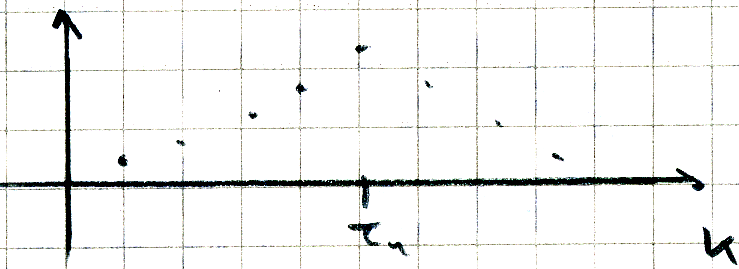
\includegraphics[width=1\textwidth]{./pics/MSTAT004.png}
		\caption{Plot von $\E[S_k]$}
		%\label{Abb}
	\end{center}
\end{figure}

Dies motiviert folgenden Schätzer (ersetze unbekannte $\big|\E[S_k]\big|$ durch bekannte $|S_k|$):
\begin{align*}
	\hat{\tau}_n:=\argmax\limits_{0\leq k\leq n}\big|S_k\big|
\end{align*}
Im Folgenden sei $\tau_n=\lfloor n\cdot\theta\rfloor,\theta\in(0,1)$.
Wir zeigen:
\begin{align*}
	\hat{\theta}_n:=\frac{\hat{\tau}_n}{n}\overset{n\to\infty}{\longrightarrow}\theta\qquad\P\text{-f.s.}
\end{align*}

\textbf{Annahme:} Wir nehmen die sogenannte \textbf{Momentenbedingung an}, d.h.
\begin{align*}
	\mu_p:=\E\Big[\big|X_{\tau_n}\big|^p\Big]<\infty,
	\qquad
	\nu_p:=\E\Big[\big|X_{\tau_n+1}\big|^p\Big]<\infty
\end{align*}

Sei $M_n:=$ Polygonzug durch $\left(\frac{k}{n},\frac{1}{n}\cdot S_k\right)$, $0\leq k\leq n$.
Dann folgt aus Lemma \ref{lemma7.17}:
\begin{align*}
	\hat{\theta}_n&:=\argmax\limits_{0\leq t\leq 1}\big|M_n(t)\big|\\
	M_n(t)&~=\frac{1}{n}\cdot S_{\lfloor n\cdot t\rfloor}+\big(n\cdot t-\lfloor w\cdot t\rfloor\big)\cdot\Big(S_{\lfloor n\cdot t\rfloor+1}-S_{\lfloor n\cdot t\rfloor+1}\Big) &\forall 0\leq t\leq 1\\
	\E\big[M_n(t)\big]&~=\frac{1}{n}\cdot\E\Big[ S_{\lfloor n\cdot t\rfloor}\Big]+\big(n\cdot t-\lfloor w\cdot t\rfloor\big)\cdot
	\Big(\E\Big[S_{\lfloor n\cdot t\rfloor+1}\Big]-\E\Big[S_{\lfloor n\cdot t\rfloor+1}\Big]\Big) &\forall 0\leq t\leq 1\\
\end{align*}

Sei $\overline{M}_n(t):=\E\big[M_n(t)\big),0\leq t\leq 1$. 
Dann ist $\overline{M}_n$ ein Polygonzug durch die Punkte $\left(\frac{k}{n},\frac{1}{n}\cdot\E[S_k]\right)$ $0\leq k\leq n$.
Da wegen \eqref{eqUnder8.2_1} 
\begin{align*}
	\overline{M}_n\left(\frac{k}{n}\right)
	&=\frac{1}{n}\cdot\E\big[S_k\big]
	\overset{\eqref{eqUnder8.2_1}}
	=
	\left\lbrace\begin{array}{cl}
		\frac{k}{n}\cdot(1-\theta_n)\cdot(\mu-\nu) &\falls \frac{k}{n}\leq\frac{\tau_n}{n}=\theta_n\\
		\left(1-\frac{k}{n}\right)\cdot\theta_n\cdot(\mu-\nu), & \falls \frac{k}{n}>\theta_n
	\end{array}\right.
\end{align*}
folgt
\begin{align*}
	\overline{M}_n\left(t\right)
	&=\left\lbrace\begin{array}{cl}
		t\cdot(1-\theta_n)\cdot(\mu-\nu) &\falls t\leq\theta_n\\
		\left(1-t\right)\cdot\theta_n\cdot(\mu-\nu), & \falls \frac{k}{n}>\theta_n
	\end{array}\right.
\end{align*}
Beachte $\theta-\frac{1}{n}<\theta_n=\frac{\lfloor n\cdot\theta\rfloor}{n}=\theta$.
Eine Fallunterscheidung ($t\leq\theta_n$; $\theta_n<t\leq\theta$; $t>\theta$) liefert
\begin{align}\label{eqUnder8.2_2}\tag{2}
	\big\Vert\overline{M}_n-M\big\Vert
	&=\sup\limits_{0\leq t\leq 1}\Big|\overline{M}_n(t)-M(t)\Big|
	\leq 2\cdot|\mu-\nu|\cdot n^{-1}\overset{n\to\infty}{\longrightarrow}0\text{ wobei}\\\nonumber
	M(t)&=\left\lbrace\begin{array}{cl}
		t\cdot(1-\theta)\cdot(\mu-\nu) ,&\falls 0\leq t\leq\theta\\
		(1-t)\cdot\theta\cdot(\mu-\nu), &\falls \theta<t\leq 1
	\end{array}\right.\\\nonumber
	|M(t)|&=\left\lbrace\begin{array}{cl}
		t\cdot(1-\theta)\cdot|\mu-\nu| ,&\falls 0\leq t\leq\theta\\
		(1-t)\cdot\theta\cdot|\mu-\nu|, &\falls \theta<t\leq 1
	\end{array}\right.
\end{align}

\begin{figure}[H]
	\begin{center}
		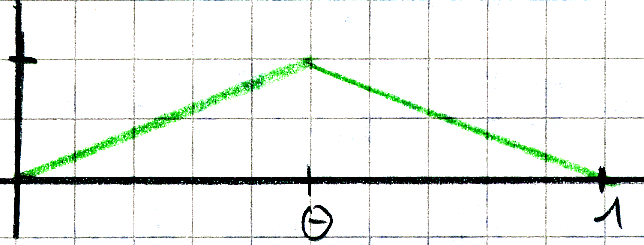
\includegraphics[width=1\textwidth]{./pics/MSTAT005.png}
		\caption{Plot von $M(t)$}
		%\label{AbbTitel}
	\end{center}
\end{figure}

Somit ist dieses $\theta$ charakterisierbar als Maximalstelle:
\begin{align*}
	\theta=\argmax\limits_{0\leq t\leq 1}\big|M(t)\big|
\end{align*}

Zeige:
\begin{align*}
	\big\Vert M_n-M\big\Vert
	&=\sup\limits_{0\leq t\leq 1}\big|M_n(t)-M(t)\big|\overset{n\to\infty}{\longrightarrow}0\quad\P\text{-f.s.}
\end{align*}
Da
\begin{align}\label{eqUnder8.2_3}\tag{3}
	0\leq\big\Vert M_n-M\big\Vert\leq\big\Vert M_n-\overline{M}_n\big\Vert+\underbrace{\big\Vert\overline{M}_n-M\big\Vert}_{
		\stackrelnew{\eqref{eqUnder8.2_2}}{n\to\infty}{\longrightarrow}0
	}
\end{align}

Betrachte den ersten Summanden
\begin{align}\label{eqUnder8.2_4}\tag{4}
	\big\Vert M_n-\overline{M}_n\big\Vert
	=\sup\limits_{0\leq t\leq 1}&\big|M_n(t)-\overline{M}_n(t)\big|
	\overset{\ref{lemma7.17}}{=}
	\max\limits_{0\leq k\leq n}\bigg|\underbrace{M_n\left(\frac{k}{n}\right)}_{=\frac{1}{n}\cdot S_k}-\underbrace{\overline{M}_n\left(\frac{k}{n}\right)}_{=\frac{1}{n}\cdot\E[S_k]}\bigg|\\\nonumber
	\frac{1}{n}\cdot S_k
	&=\frac{1}{n}\cdot\sum\limits_{i=1}^k\big(X_i-\overline{X}_n\big)
	=\frac{1}{n}\cdot\sum\limits_{i=1}^k X_i-\frac{k}{n^2}\cdot\sum\limits_{i=1}^n X_i\\\nonumber
	\implies
	M_n\left(\frac{k}{n}\right)-\overline{M}_n\left(\frac{k}{n}\right)
	\overset{\text{Lin}}&=
	\frac{1}{n}\cdot\sum\limits_{i=1}^n\underbrace{\Big(X_i-\E\big[X_i\big]\Big)}_{=:Z_i}-\frac{k}{n^2}\cdot\sum\limits_{i=1}^n\underbrace{\Big(X_i-\E\big[X_i\big]\Big)}_{=Z_i}\\\nonumber
	\implies
	\left|M_n\left(\frac{k}{n}\right)-\overline{M}_n\left(\frac{k}{n}\right)\right|
	\overset{\text{DU}}&\leq
	\frac{1}{n}\cdot\underbrace{\bigg|\sum\limits_{i=1}^n\underbrace{\Big(X_i-\E\big[X_i\big]\Big)}_{=:Z_i}\bigg|}_{
		\leq\max\limits_{0\leq k\leq n}\left|\sum\limits_{i=1}^k Z_i\right|
	}+\underbrace{\frac{k}{n^2}}_{\leq\frac{1}{n}}\underbrace{\cdot\bigg|\sum\limits_{i=1}^n\underbrace{\Big(X_i-\E\big[X_i\big]\Big)}_{=Z_i}\bigg|}_{
		\leq\max\limits_{0\leq k\leq n}\left|\sum\limits_{i=1}^k Z_i\right|
	}\\\nonumber
	&\leq2\cdot\frac{1}{n}\cdot\max\limits_{0\leq k\leq n}\left|\sum\limits_{i=1}^k Z_i\right|\\
	\implies\label{eqUnder8.2_5}\tag{5}
	&\max\limits_{0\leq k\leq n}\left|M_n\left(\frac{k}{n}\right)-\overline{M}_n\left(\frac{k}{n}\right)\right|
	\leq 2\cdot\frac{1}{n}\cdot\max\limits_{0\leq k\leq n}\left|\sum\limits_{i=1}^k Z_i\right|
\end{align}

Es ist
\begin{align*}
	T_k=\sum\limits_{i=1}^k Z_i\qquad 0\leq k\leq n
\end{align*}
ein Martingal bzgl. Filtration 
\begin{align*}
	\F_k:=\sigma\big(Z_1,\ldots,Z_k\big) &\qquad\forall 1\leq k\leq n,\qquad \F_0:=\lbrace\emptyset,\Omega\rbrace
\end{align*}
Ist Martingal, weil
\begin{align*}
	\E\Big[T_{k+1}~\Big|~\F_k\Big]
	&=\E\left.\left[\sum\limits_{i=1}^k Z_i+Z_{k+1}~\right|~\F_k\right]
	=\underbrace{\E\bigg[\overbrace{\sum\limits_{i=1}^k Z_i}^{\text{ist $\F_K$-messbar}}~\bigg|~\F_k\bigg]}_{=T_k}+\underbrace{\E\Big[ Z_{k+1}~\Big|~\F_k\Big]}_{=\E[Z_{k+1}]=0}
\end{align*}

Es folgt aus der bedingten Jensenungleichung, dass $\left(|T_k|^p,\F_k\right)_{0\leq k\leq n}$ ein nicht-negatives Submartingal ist.
\begin{align}\nonumber
	\P\Big(\big\Vert M_n-\overline{M}_n\big\Vert\geq\varepsilon\Big)
	\overset{\eqref{eqUnder8.2_4}+\eqref{eqUnder8.2_5}}&{\leq}
	2\cdot\frac{1}{n}\cdot\max\limits_{0\leq k\leq n}\big|T_k\big|\\\nonumber
	&\leq\P\left(\max\limits_{0\leq k\leq n}\big|T_k\big|\geq\frac{1}{2}\cdot n\cdot\varepsilon\right)\\\nonumber
	\overset{u\mapsto u^p\uparrow}&\leq
	\P\left(\left(\max\limits_{0\leq k\leq n}\big|T_k\big|\right)^p\geq\left(\frac{1}{2}\cdot n\cdot\varepsilon\right)^p\right)\\\nonumber
	&=\P\left(\max\limits_{0\leq k\leq n}\big|T_k\big|^p\geq\left(\frac{1}{2}\cdot n\cdot\varepsilon\right)^p\right)\\\nonumber
	\implies
	\P\Big(\big\Vert M_n-\overline{M}_n\big\Vert\geq\varepsilon\Big)
	&\leq\P\bigg(\max\limits_{0\leq k\leq n}\underbrace{\big|T_k\big|^p}_{\text{Submartingal}}\geq\underbrace{2^{-p}\cdot n^p\cdot\varepsilon^p}_{=:y>0}\bigg)\\\nonumber
	\overset{\text{Doob-Ungl}}&\leq
	y^{-1}\cdot\E\left[\big|T_n\big|^p\right]\\
	&=2^p\cdot n^{-p}\cdot\varepsilon^{-p}\cdot\E\left[\left|\sum\limits_{i=1}^n Z_i\right|^p\right]\label{eqUnder8.2_6}\tag{6}
\end{align}

Es gilt folgende \textbf{Momenten-Ungleichung} (vergleiche (1.6) in Ferger (2014), \textit{Optimal constants in the Marcinkiewicz-Zygmund-inequalities, statistics and propability letters} Ausgabe 84, Seiten 96 bis 101)

\begin{align*}
	\E\left[\left|\sum\limits_{i=1}^n Z_i\right|^p\right]
	\overset{(1.6)}{\leq}
	C_p\cdot n^{\frac{p}{2}}\cdot\sum\limits_{i=1}^n\E\Big[|Z_i|^p\Big]
\end{align*}

Erinnerung:
\begin{align*}
	Z_i&=X_i-\E[X_i]\\
	\implies
	|Z_i|^p&=\big|X_i-\E[X_i]\big|^p\\
	\implies
	\big|X_i-\E[X_i]\big|^p
	\overset{C_r\text{ Ungl}}&\leq
	c_p\cdot\Big(|X_i|^p+\underbrace{\big|\E[X_i]\big|^p}_{\overset{\text{Jensen}}{\leq}\E\big[|X_i|^p\big]}\Big)\\
	\implies
	\E\Big[|Z_i|^p\Big]
	&\leq c_p\cdot\left(\E\big[|X_i|^p\big]+\E\big[|X_i|^p\big]\right)\\
	&\leq 2\cdot c_p\cdot\underbrace{\E\Big[|X_i|^p\Big]}_{\leq\max\lbrace\mu_p,\nu_p\rbrace}
\end{align*}
Somit gibt es eine Konstante $D_p$ so, dass
\begin{align*}
	\E\left[\left|\sum\limits_{i=1}^n Z_i\right|^p\right]
	\overset{(1.6)}&{\leq}
	C_p\cdot n^{-\frac{p}{2}}\cdot\sum\limits_{i=1}^n\underbrace{\E\Big[|Z_i|^p\Big]}_{\leq D_p}\\
	\implies
	\E\left[\left|\sum\limits_{i=1}^n Z_i\right|\right]
	&\leq\tilde{c}_p\cdot n^{\frac{p}{2}}\\
	\overset{\eqref{eqUnder8.2_6}}{\implies}
	\P\Big(\big\Vert M_m-\overline{M}_n\big\Vert\geq\varepsilon\Big)
	&\leq\overline{c}_p\cdot\varepsilon^{-p}\qquad\forall\varepsilon>0
\end{align*}

Nun bilden wir die Reihe dieser Wahrscheinlichkeiten und erhalten Konvergenz für $p>2$:
\begin{align*}
	\overset{p>2}{\implies}
	\sum\limits_{n=1}^\infty\P\Big(\big\Vert M_m-\overline{M}_n\big\Vert\geq\varepsilon\Big)<\infty\qquad\forall\varepsilon>0
\end{align*}

Es gilt ganz allgemein für eine Folge $(\xi_n)_{n\in\N}$ von Zufallsvariablen (folgt aus dem Borel-Cantelli-Lemma):
\begin{align*}
	\left(\forall\varepsilon>0:\sum\limits_{n=1}^\infty\P\Big(|\xi_n|\geq\varepsilon\Big)<\infty\right)\implies\xi_n\overset{n\to\infty}{\longrightarrow}0\text{ f.s.}
\end{align*}

Also erhalten wir
\begin{align*}
	\big\Vert M_n-\overline{M}_n\big\Vert\overset{n\to\infty}{\longrightarrow}0\text{ f.s.}\\
	\overset{\eqref{eqUnder8.2_2}+\eqref{eqUnder8.2_3}}{\implies}
	\big\Vert M_n-M\big\Vert\overset{n\to\infty}{\longrightarrow}0\text{ f.s.}
\end{align*}

Da
\begin{align*}
	\Big\Vert\big|M_n\big|-\big|M\big|\Big\Vert\leq\big\Vert M_n-M\big\Vert
\end{align*}
folgt
\begin{align*}
	\Big\Vert\big|M_n\big|-\big|M\big|\Big\Vert\overset{n\to\infty}&{\longrightarrow}0\text{ f.s.}\\
	\implies	
	\Big\Vert-\big|M_n\big|-\big(-\big|M\big|)\Big\Vert\overset{n\to\infty}&{\longrightarrow}0\text{ f.s.}\\
	\implies
	\hat{\theta}_n
	&=\argmax\limits_{0\leq t\leq 1}\big|M_n(t)\big|
	=\argmin\limits_{0\leq t\leq 1}-\big|M_n(t)\big|
\end{align*}
Also hat $-|M|$ eindeutige Minimalstelle $\theta$.
Aus Satz \ref{satz8.6} folgt nun $\hat{\theta}\overset{n\to\infty}{\longrightarrow}\theta$ f.s.\\
(In Satz \ref{satz8.6} verwende: $M_n\hat{=}-|M_n|$, $M\hat{=}|M|$, $\tau\hat{=}\theta$)

\begin{bemerkung}
	Betrachte eine endliche Beobachtungsfolge:\\
	$X_1,X_2,\ldots,X_\tau,X_{\tau+1},X_{\tau+},\ldots,X_n\qquad n>\tau$\\
	Hier braucht man keinen doppelten Index.
	Vergrößert man aber nun $n$, dann geht der Anteil an der Gesamtstichprobe gegen 0, also $\frac{\tau}{n}\longrightarrow0$.
\end{bemerkung}

Zusammenfassung unserer Überlegungen in
\begin{satz}\label{satz8.8}
	Sei $\theta\in(0,1),\mu\neq\nu,\mu_p<\infty,\nu_p<\infty$ für ein $p>2$.
	Dann gilt:
	\begin{align*}
		\hat{\theta}_n
		&=\frac{1}{n}\cdot\underbrace{\argmax\limits_{0\leq k\leq n}\left|\sum\limits_{i=1}^k\big(X_i-\overline{X}_n\big)\right|}_{=\hat{\tau}_n}\overset{n\to\infty}{\longrightarrow}0\text{ f.s.}
	\end{align*}
\end{satz}

\begin{bemerkung}
	 Es gilt \underline{nicht}, dass $\hat{\tau}_n-\tau_n\overset{n\to\infty}{\longrightarrow}0$ f.s.
	 Tatsächlich gilt:
	 \begin{align*}
	 	\hat{\tau}_n-\tau_n\overset{\L}{\longrightarrow} T
	 \end{align*}
	 wobei $T$ die f.s. eindeutige Maximalstelle einer \textit{2-seitigen Irrfahrt / Random Walk} auf $\Z$ ist
	 (vergleiche D.F. (1994) \textit{Asymptotic distribution theory of change-point estimators} veröffentlicht in \textit{Mathematical methods in statics 3}, Seiten 362 bis 378).
\end{bemerkung}

Nächstes Ziel: Unter welchen Bedingungen gilt
\begin{align*}
	Z_n\overset{L}{\longrightarrow}Z\text{ in }\big(C(\R),d\big)
	\implies\argmin\limits_{t\in\R}Z_n(t)\overset{\L}{\longrightarrow}\argmin\limits_{t\in\R}Z(t)
\end{align*}

Folgender Satz gibt Antwort.

\begin{satz}\label{satz8.9}
	Seien $Z,Z_n,n\in\N$ stochastische Prozesse mit Pfaden in $C(\R)$ über $(\Omega,\A,P)$,
	wobei $A(Z)$ 
	\footnote{$A(Z)$ ist eine \textit{random closed set (RCS)}} 
	und $A(Z_n)$ für alle $n\in\N$ nichtleer sind.
	Ferner sei $\sigma_n$ eine Zufallsvariable mit $\sigma_n\in A(Z_n)$.
	Dann gilt: Falls
	\begin{align}\label{eqSatz8.9_1}\tag{1}
		Z_n\overset{\L}{\longrightarrow} Z\text{ in }\big(C(\R),d\big)
	\end{align}
	so folgt
	\begin{align}\label{eqSatz8.9_a}\tag{a}
		\limsup\limits_{n\to\infty}\P\big(\sigma_n\in K\big)\leq\mu^\ast(K)\qquad\forall K\in\mathcal{K}:=\big\lbrace K\subseteq\R:K\text{ kompakt}\big\rbrace
	\end{align}
	wobei $\mu^\ast$
	\footnote{$\mu^\ast$ ist die \textit{Kapazitätsfunktion von $A(Z)$} und damit insbesondere eine \textit{Choquet-Kapazität}.
	Beachte, dass $\mu^\ast$ i.d.R. \underline{kein} W-Maß.}	
	die sogenannte \textbf{hitting-probability} ist:
	\begin{align*}
		\mu^\ast:\mathcal{K}\to[0,1],\qquad
		\mu^\ast(K)=\P\big(A(Z)\cap K\neq\emptyset\big)
	\end{align*}
	Gilt zusätzlich, dass $(\sigma_n)_{n\in\N}$ \textbf{stochastisch beschränkt} ist, d.h. 
	\begin{align}\label{eqSatz8.9_2}\tag{2}
		\lim\limits_{j\to\infty}\limsup\limits_{n\to\infty}\P\Big(\big|\sigma_n\big|>j\Big)=0
	\end{align}
	so folgt
	\begin{align}\label{eqSatz8.9_b}\tag{b}
		\limsup\limits_{n\to\infty}\P\big(\sigma_n\in F\big)\leq\mu^\ast(F)\qquad\forall F\in\F(\R):=\big\lbrace F\subseteq\R:F\text{ abgeschlossen}\big\rbrace
	\end{align}
	Falls zusätzlich $A(Z)=\lbrace\sigma\rbrace$ für eine Zufallsvariable $\sigma$
	(d.h. $Z$ hat f.s. eine eindeutige Minimalstelle, nämlich $\sigma$), dann gilt
	\begin{align}\label{eqSatz8.9_c}\tag{c}
		\sigma_n\overset{\L}{\longrightarrow}\sigma\text{ in }\R.
	\end{align}
\end{satz}

%Ferger: "Ich weiß nicht mehr wie ich drauf gekommen bin. Aber ich bin darauf gekommen. Da habe ich mich gefreut wie so ein Brötchen."
%Ferger: "Müssen Sie nicht mitschreiben, ich will jetzt hier nur zu einer didaktischen Meisterleistung auflaufen."

\begin{proof}
	\underline{Zeige \eqref{eqSatz8.9_a}:}\\
	Sei $K$ kompakt. Dann gilt:
	\begin{align}\label{eqProofSatz8.9_i}\tag{i}
		\big\lbrace\sigma_n\in K\big\rbrace
		&\subseteq\left\lbrace\inf\limits{t\in K} Z_n(t)\leq\inf\limits_{t\not\in K} Z_n(t)\right\rbrace\\
		&\subseteq\left\lbrace\inf\limits_{t\in K} Z_n(t)\leq\inf\limits_{t\in K^C\cap I_j}Z_n(t)\right\rbrace\label{eqProofSatz8.9_ii}\tag{ii}
	\end{align}
	wobei $I_j:=[-j,j],j\in\N$.\nl
	\underline{Zeige \eqref{eqProofSatz8.9_i}:}\\
	Sei $\sigma_n\in K$ und angenommen
	\begin{align}\label{eqProofSatz8.9Stern}\tag{$\ast$}
		\inf\limits_{t\in K} Z_n(t)>\inf\limits_{t\in K^C} Z_n(t)
	\end{align}
	Dann gilt:
	\begin{align*}
		Z_n(\sigma_n)
		\overset{\sigma_n\in K}&\geq
		\inf\limits_{t\in K} Z_n(t)
		\overset{\eqref{eqProofSatz8.9Stern}}>
		\inf\limits_{t\in K^C} Z_n(t)
		\overset{K^C\subseteq\R}\geq
		\inf\limits_{t\in\R} Z_n(t)
		\overset{\sigma_n\in A(Z_n)}=
		Z(\sigma_n)
	\end{align*}
	Das ist ein Widerspruch, weshalb \eqref{eqProofSatz8.9_i} folgt.\nl
	Gleichung \eqref{eqProofSatz8.9_ii} folgt aus 
	\begin{align*}
		\inf\limits_{t\in K^C} Z_n(t)\leq\inf\limits_{t\in K^C\cap I_j}Z_n(t).
	\end{align*}
	Sei $K_j:=[-k_j,k_j]$ mit $k_j\in\N$ so, dass $K_j\supseteq K\cup I_j$.
	Für jedes $M\subseteq K_j$ gilt:
	Die Abbildung $f\mapsto\inf\limits_{t\in M} f(t)$ ist stetig auf $\big(C(K_j),\Vert\cdot\Vert_{K_j}\big)$,
	denn:
	\begin{align*}
		\left|\inf\limits_{t\in M} f(t)-\inf\limits_{t\in M}g(t)\right|
		&\leq \Vert f-g\Vert_M
		\leq\Vert f-g\Vert_{K_j}
	\end{align*}
	Daraus folgt, dass die Abbildung
	\begin{align*}
		H_j:\left(C\big(K_j\big),\Vert\cdot\Vert_{K_j}\right)\to\R,\qquad
		f\mapsto\inf\limits_{t\in K} f(t)-\inf\limits_{t\in K^C\cap I_j} f(t)
	\end{align*}
	stetig ist, denn $K^C\cap I_j\subseteq I_j\subseteq K\cup I_j\subseteq K_j$.
	Somit folgt aus Satz \ref{satz7.23} und aus dem CMT \ref{satz4.10ContinuousMappingTheorem}:
	\begin{align}\label{eqProofSatz8.9_iii}\tag{iii}
		H_j(Z_n)\overset{\L}{\longrightarrow} H_j(Z)\qquad\forall j\in\N
	\end{align}
	Aus \eqref{eqProofSatz8.9_i} und \eqref{eqProofSatz8.9_ii} folgt:
	\begin{align}\nonumber
		\P\Big(\big\lbrace\sigma_n\in K\big\rbrace\Big)
			&\leq\P\Bigg(\Bigg\lbrace\underbrace{\inf\limits_{t\in K} Z_n(t)-\inf\limits_{t\in K^C\cap I_j}Z_n(t)}_{=H_j(Z_n)}\leq0\Bigg\rbrace\Bigg)\\\nonumber
		\implies		
		\limsup\limits_{n\to\infty}\P\big(\sigma_n\in K\big)
		\overset{\eqref{eqProofSatz8.9_i}+\eqref{eqProofSatz8.9_ii}}&\leq
		\limsup\limits_{n\to\infty}\P\Big(H_j(Z_n)\in\underbrace{(-\infty,0]}_{\in\F(\R)}\Big)\\\nonumber
		\overset{\eqref{eqProofSatz8.9_iii}+\text{Portmannteau}}&\leq
		\P\Big(H_j(Z)\in(-\infty,0]\Big)\\
		\overset{\text{Def }H_j}&=
		\P\bigg(\underbrace{\bigg\lbrace\inf\limits_{t\in K}Z(t)\leq\inf\limits_{t\in K^C\cap I_j}Z(t)\bigg\rbrace}_{=:E_j}\qquad\forall j\in\N\label{eqProofSatz8.9_iv}\tag{iv}
	\end{align}
	Da $E_j$ monoton fallend ist, folgt (mit $\sigma$-Stetigkeit von oben):
	\begin{align*}
		\lim\limits_{j\to\infty}\P(E_j)
		&=\P\left(\bigcap\limits_{j\in\N}E_j\right)\\
		&=\P\left(\inf\limits_{t\in K}Z(t)\leq\inf\limits_{t\in K^C\cap I_j}Z(t)~\forall j\in\N\right)\\
		&\leq \P\bigg(\inf\limits_{t\in K}Z(t)\leq\underbrace{\inf\limits_{j\in\N}\inf\limits_{t\in K^C\cap I_j}Z(t)}_{=\inf\limits_{\bigcup\limits_{j\in\N}\big(K^C\cap I_j\big)}Z(t)}\bigg)\\
		\overset{\bigcup\limits_j(K^C\cap I_j)=K^C\cap\bigcap\limits_j I_j=K^C\cap\R}&=
		\P\bigg(\underbrace{\bigg\lbrace\inf\limits_{t\in K} Z(t)\leq\inf\limits_{t\in K^C} Z(t)\bigg\rbrace}_{=:E}\bigg)
	\end{align*}
	Dahinter steckt die allgemeine Rechenregel
	\begin{align*}
		\inf\limits_{t\in A\cup B}f(t)=\inf\limits\left\lbrace\inf\limits_A f,\inf\limits_B f\right\rbrace.
	\end{align*}
	Grenzübergang $j\to\infty$ in \eqref{eqProofSatz8.9_iv} liefert:
	\begin{align}\label{eqProofSatz8.9Plus}\tag{+}
		\limsup\limits_{n\to\infty}\P\big(\sigma_n\in K\big)
		\leq\lim\limits_{j\to\infty}\P(E_j)\leq\P(E)
	\end{align}
	Schließlich gilt
	\begin{align}\label{eqProofSatz8.9_v}\tag{v}
		E\subseteq\big\lbrace A(Z)\cap K\neq\emptyset\big\rbrace
	\end{align}
	denn:
	\begin{align*}
		&\inf\limits_{t\in K}Z(t)
		\leq\inf\limits_{t\in K^C} Z(t)\\
		&\implies
		\inf\limits_\R Z(t)=\inf\limits_{K\cup K^C}Z(t)=\min\left\lbrace\inf\limits_{t\in K} Z(t),\inf\limits_{t\in K^C}Z(t)\right\rbrace=\inf_{t\in K}Z(t)
		=Z(\tau)
	\end{align*}
	für ein $\tau\in K$, da $Z$ stetig und $K$ kompakt.
	Also ist $\tau$ eine Minimalstelle von $Z$, i.Z. $\tau\in A(Z)$.
	Da $\tau\in K$ ist, gilt
	\begin{align*}
		\tau\in A(Z)\cap K\\
		\implies A(Z)\cap K\neq\emptyset
	\end{align*}
	Wegen \eqref{eqProofSatz8.9_v} gilt, dass
	\begin{align*}
		\P(E)\leq\P\big(A(Z)\cap K\neq\emptyset\big)=\mu^\ast(K)
	\end{align*}
	und \eqref{eqSatz8.9_a} folgt aus \eqref{eqProofSatz8.9Plus}.\nl
	\underline{Zeige \eqref{eqSatz8.9_b}:}\\
	Sei $F\in\F$. Dann gilt:
	\begin{align}\nonumber
		\big\lbrace\sigma_n\in F\big\rbrace
		\overset{\text{Zerlegung}}&=
		\big\lbrace\sigma_n\in F,\sigma_n\in I_j\big\rbrace
		\dot{\cup}\big\lbrace\sigma_n\in F,\sigma_n\not\in I_j\big\rbrace\\\nonumber
		&=\big\lbrace\sigma_n\in \underbrace{F\cap I_j}_{\text{kompakt}}\big\rbrace\dot{\cup}\big\lbrace |\sigma_n|>j\big\rbrace&\forall& j\in\N\\\nonumber
		\implies
		\P\Big(\big\lbrace\sigma_n\in F\big\rbrace\Big)
		&\leq\P\Big(\big\lbrace\sigma_n\in F\cap I_j\big\rbrace\Big)+\P\Big(\big\lbrace |\sigma_n|>j\big\rbrace\Big)&\forall& j\in\N\\
		\limsup\limits_{n\to\infty}\P(\sigma_n\in F)
		&\leq\underbrace{\limsup\limits_{n\to\infty}\P\big(\sigma_n\in F\cap I_j)}_{
			\overset{\eqref{eqSatz8.9_a}}{\leq}\P\big(\underbrace{\big\lbrace A(Z)\cap(F\cap I_j)\neq\emptyset\big\rbrace}_{=:B_j}
		}+\underbrace{\limsup\limits_{n\to\infty}\P\big(|\sigma_n|>j\big)}_{
			\overset{j\to\infty}{\longrightarrow}\text{ wegen }\eqref{eqSatz8.9_2}
		} &\forall& j\in\N\label{eqProofSatz8.9PlusPlus}\tag{++}
	\end{align}
	Da
	\begin{align*}
		B_j\uparrow\big\lbrace A(Z)\cap F\neq\emptyset\big\rbrace
	\end{align*}
	 (zur Übung), liefert Grenzübergang $j\to\infty$ in \eqref{eqProofSatz8.9PlusPlus} und $\sigma$-Stetigkeit von unten und \eqref{eqSatz8.9_2} die Behauptung \eqref{eqSatz8.9_b}.\nl
	 \underline{Zeige \eqref{eqSatz8.9_c}:}
	 \begin{align*}
	 	&A(Z)=\lbrace\sigma\rbrace\text{ f.s.}\\
	 	&\implies\mu^\ast(F)=\P\big(A(Z)\cap F\neq\emptyset\big)
	 	=\P\Big(\big\lbrace\sigma\rbrace\cap F\neq\emptyset\big\rbrace\Big)
	 	=\P(\sigma\in F)\\
	 	\overset{\eqref{eqSatz8.9_b}}&\implies
	 	\limsup\limits_{n\to\infty}\P\big(\sigma_n\in F\big)\leq\mu^\ast(F)
	 	=\P(\sigma\in F)\qquad\forall F\in F\\
	 	\overset{\text{Portmannteau}}&{\implies}
	 	\sigma_n\overset{\L}{\longrightarrow}\sigma
	 \end{align*}
\end{proof}

%Ferger: "Ich war früher so ein richtiger Sport-Paul. Aber jetzt bin ich einfach zu faul. Ist nicht so, dass ich keine Zeit habe.

\subsection{Anwendung}

Sei $X_1,\ldots,X_n$ i.i.d. Kopien von $X$ mit $\mu$-Dichte 
\begin{align*}
	f_\theta(x)&=c(\theta)\cdot h(x)\cdot\exp\big(q(\theta)\cdot T(x)\big)\qquad\forall x\in\X,\forall\theta\in\Theta=\R
\end{align*}
Sei $\theta_0$ der wahre Parameter.
Dann gilt:

\begin{align}\label{eqAnwendung_1}\tag{1}
	\text{MLS $\hat{\theta}_n$ für $\theta$ ist }\hat{\theta}_n&=\argmin\limits_{t\in\R}M_n(t)\qquad\mit\\
	M_n(t)&=-\log\big(c(t)\big)-q(t)\cdot\overline{T}_n,\qquad
	\overline{T}_n=\frac{1}{n}\cdot\sum\limits_{i=1}^nt(X_i)\nonumber
\end{align}
Ziel: Nachweis von
\begin{align*}
	\sqrt{n}\cdot\big(\hat{\theta}_n-\theta_0\big)\overset{\L}{\longrightarrow}\xi
\end{align*}
und Identifizierung von $\xi$.\nl
Dazu: Sei 
\begin{align*}
	Z_n(t):=n\cdot\left(M_n\left(\theta_0+\frac{t}{\sqrt{n}}\right)-M_n\big(\theta_0\big)\right)\qquad\forall t\in\R
\end{align*}
der \textbf{reskalierte Prozess} zu $M_n$.
Offenbar ist $Z_n$ stetiger stochastischer Prozess \underline{und}
\begin{align}\label{eqAnwendung_2}\tag{2}
	\underbrace{\sqrt{n}\cdot\big(\hat{\theta}_n-\theta\big)}_{=:\sigma_n}
	&=\argmin\limits_{t\in\R} Z_n(t)
\end{align}
denn:
Zu zeigen: 
\begin{align*}
	Z_n(\sigma_n)\leq Z_n(t)\qquad\forall t\in\R
\end{align*}
Dazu nutze Äquivalenzen:
\begin{align*}
	&Z_n(\sigma_n)\leq Z_n(t) &\forall& t\in\R\\
	\overset{t=\sigma_n}&\Longleftrightarrow
	n\bigg(M_n\cdot\bigg(\underbrace{\theta_0+\frac{\sigma_n}{\sqrt{n}}}_{
		\begin{subarray}{c}
			=\theta_0+\frac{\sqrt{n}\big(\hat{\theta}_n-\theta_n\big)}{\sqrt{n}}\\
			=\theta_n
		\end{subarray}
	}\bigg)-M_n(\theta_0)\bigg)
	\leq n\cdot\left(M_n\left(\theta_0+\frac{t}{\sqrt{n}}\right)-M_n(\theta_0)\right)&\forall& t\in\R\\
	&\Longleftrightarrow n\cdot\Big(M_n\big(\hat{\theta}_n\big)-M_n\big(\theta_0\big)\Big)
	\leq n\cdot\left(M_n\left(\theta_0+\frac{t}{\sqrt{n}}\right)-M_n(\theta_0)\right) &\forall&t\in\R\\
	&\Longleftrightarrow M_n\big(\hat{\theta}_n\big)
	\leq M_n\left(\theta_0+\frac{t}{\sqrt{n}}\right) &\forall&t\in\R\\
	&\Longleftrightarrow M_n\big(\hat{\theta}_n\big)
	\leq M_n\left(\theta_0+\frac{t}{\sqrt{n}}\right) &\forall& t\in\R\\
	&\Longleftrightarrow M_n\big(\hat{\theta}_n\big)\leq M_n(u) &\forall& u\in\R\\
	\overset{\eqref{eqAnwendung_1}}&\Longleftrightarrow \text{ True}
\end{align*}
Wegen \eqref{eqAnwendung_2} versuche Satz \ref{satz8.9} anzuwenden:\\
Man kann zeigen:
\begin{align}\label{eqAnwendung_i}\tag{i}
	Z_n\overset{\L}{\longrightarrow} Z\text{ in }\big(C(\R),d\big)
\end{align}
wobei
\begin{align*}
	Z(t)
	&=-q'(\theta_0)\cdot N\cdot t+\frac{1}{2}\cdot\big(q'(\theta_0)\big)^2\cdot\sigma^2(\theta_0)\cdot t^2 \qquad\forall t\in\R
\end{align*}
wobei wir fordern:
\begin{align*}
	\sigma^2(\theta_0):=\Var_{\theta_0}\big(T(X)\big)\overset{\text{Forderung}}&>0\\
	q'(\theta_0)\overset{\text{Forderung}}&\neq0\\
	N&\sim\Nor\big(0,\sigma^2(\theta_0)\big)
\end{align*}
Also ist $Z$ eine zufällige nach oben geöffnete Parabel.

\begin{align*}
	0
	&=Z'(t)
	=-q'(\theta_0)\cdot N+\big(q'(\theta_0)\big)^2\cdot\sigma^2(\theta_0)\cdot t\\
	\xi
	&=\frac{1}{q'(\theta_0)\cdot\sigma^2(\theta_0}\cdot N
	\text{ ist die eindeutige Minimalstelle von }Z.
\end{align*}
Man kann zeigen:
\begin{align*}
	\limsup\limits_{n\to\infty}\P\Big(\sqrt{n}\cdot\big|\hat{\theta}_n-\theta_0\big|\geq j\Big)
	\leq\frac{4}{\big(q'(\theta_0)\big)^2\cdot\sigma^2(\theta_0)}\cdot\frac{1}{j^2}\qquad\forall n\in\N
\end{align*}
Grenzübergang $j\to\infty$ liefert, dass zweite Bedingung \eqref{eqSatz8.9_2} in Satz \ref{satz8.9} erfüllt ist.
Somit liefert Satz \ref{satz8.9}:
\begin{align*}
	\sqrt{n}\cdot\big(\hat{\theta}_n-\theta_0\big)\overset{\L}{\longrightarrow}\xi
\end{align*}
